% Created by tikzDevice version 0.12 on 2019-03-11 09:44:28
% !TEX encoding = UTF-8 Unicode
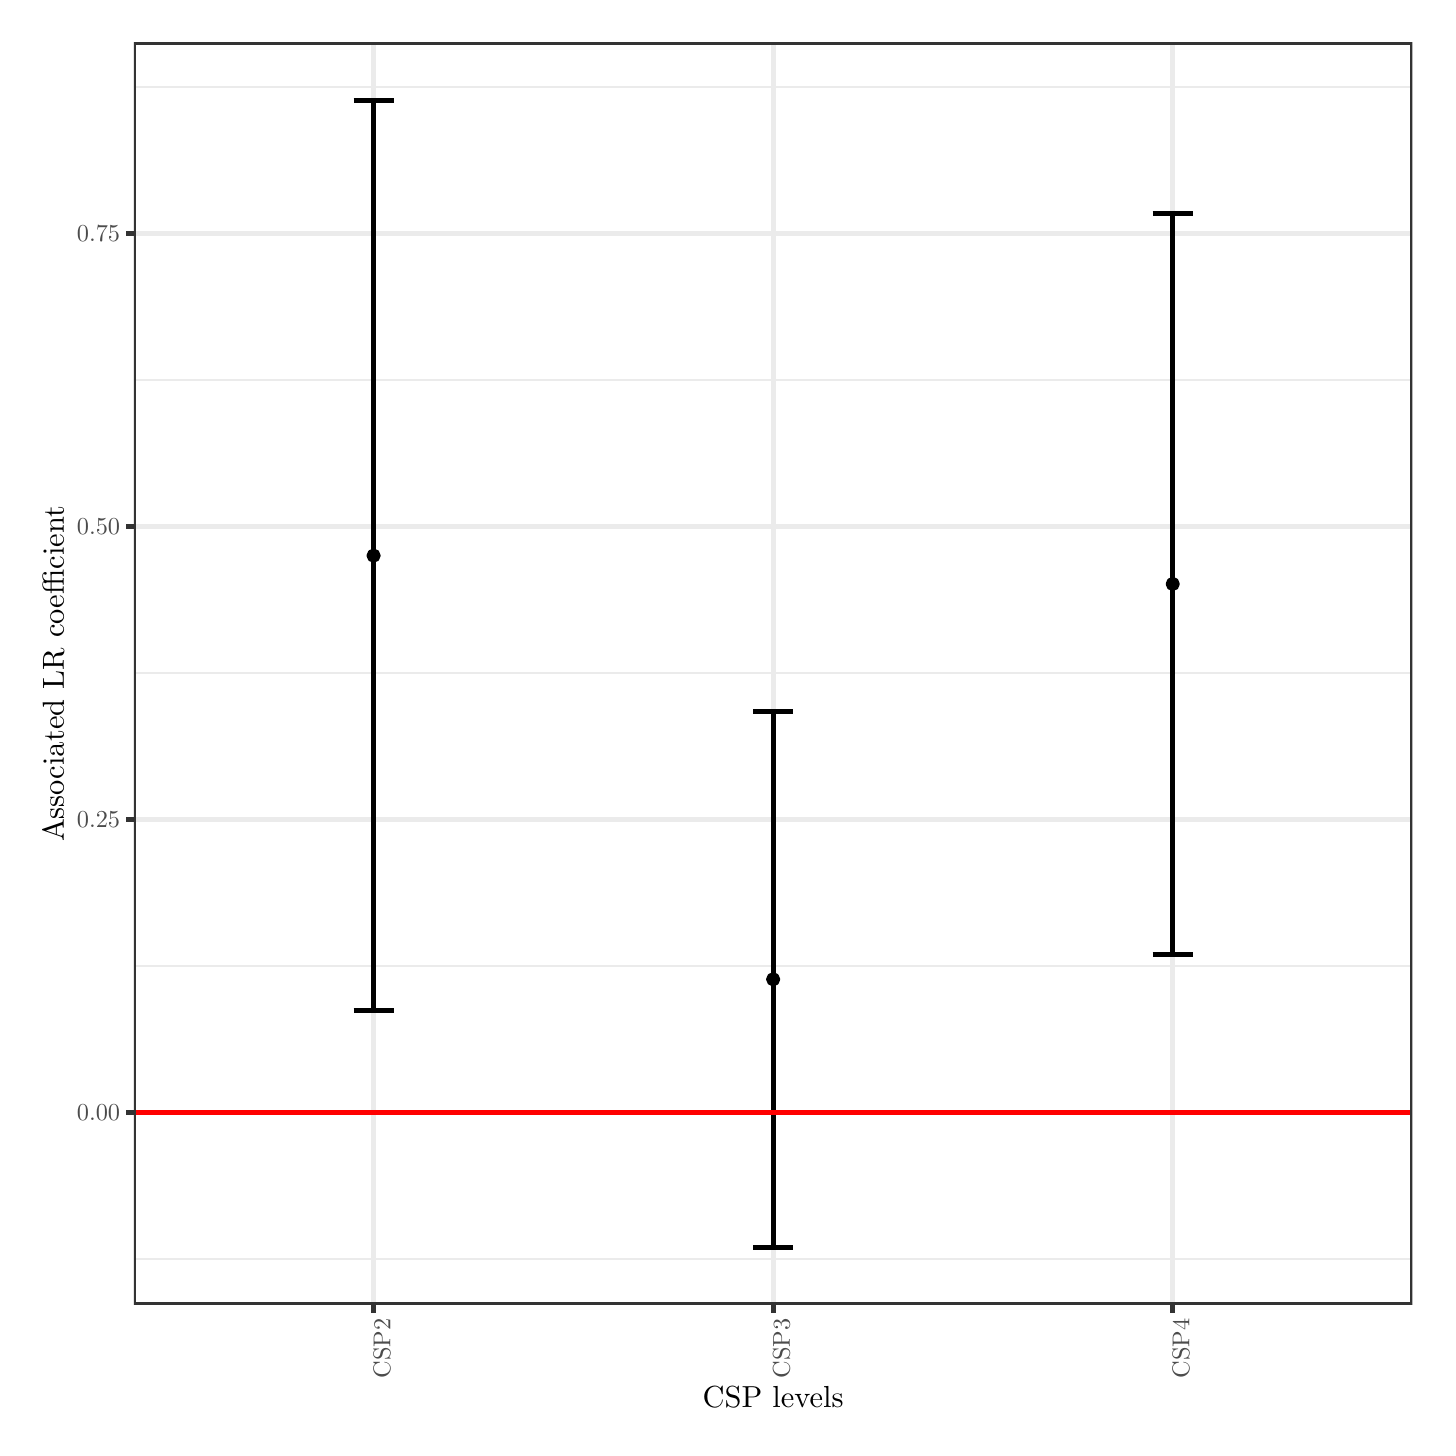
\begin{tikzpicture}[x=1pt,y=1pt]
\definecolor{fillColor}{RGB}{255,255,255}
\path[use as bounding box,fill=fillColor,fill opacity=0.00] (0,0) rectangle (505.89,505.89);
\begin{scope}
\path[clip] (  0.00,  0.00) rectangle (505.89,505.89);
\definecolor{drawColor}{RGB}{255,255,255}
\definecolor{fillColor}{RGB}{255,255,255}

\path[draw=drawColor,line width= 1.8pt,line join=round,line cap=round,fill=fillColor] (  0.00,  0.00) rectangle (505.89,505.89);
\end{scope}
\begin{scope}
\path[clip] ( 38.36, 44.35) rectangle (500.39,500.39);
\definecolor{fillColor}{RGB}{255,255,255}

\path[fill=fillColor] ( 38.36, 44.35) rectangle (500.39,500.39);
\definecolor{drawColor}{gray}{0.92}

\path[draw=drawColor,line width= 0.9pt,line join=round] ( 38.36, 60.90) --
	(500.39, 60.90);

\path[draw=drawColor,line width= 0.9pt,line join=round] ( 38.36,166.79) --
	(500.39,166.79);

\path[draw=drawColor,line width= 0.9pt,line join=round] ( 38.36,272.69) --
	(500.39,272.69);

\path[draw=drawColor,line width= 0.9pt,line join=round] ( 38.36,378.58) --
	(500.39,378.58);

\path[draw=drawColor,line width= 0.9pt,line join=round] ( 38.36,484.48) --
	(500.39,484.48);

\path[draw=drawColor,line width= 1.8pt,line join=round] ( 38.36,113.85) --
	(500.39,113.85);

\path[draw=drawColor,line width= 1.8pt,line join=round] ( 38.36,219.74) --
	(500.39,219.74);

\path[draw=drawColor,line width= 1.8pt,line join=round] ( 38.36,325.64) --
	(500.39,325.64);

\path[draw=drawColor,line width= 1.8pt,line join=round] ( 38.36,431.53) --
	(500.39,431.53);

\path[draw=drawColor,line width= 1.8pt,line join=round] (124.99, 44.35) --
	(124.99,500.39);

\path[draw=drawColor,line width= 1.8pt,line join=round] (269.38, 44.35) --
	(269.38,500.39);

\path[draw=drawColor,line width= 1.8pt,line join=round] (413.76, 44.35) --
	(413.76,500.39);
\definecolor{drawColor}{RGB}{0,0,0}

\path[draw=drawColor,line width= 1.8pt,line join=round] (117.77,479.66) --
	(132.21,479.66);

\path[draw=drawColor,line width= 1.8pt,line join=round] (124.99,479.66) --
	(124.99,150.57);

\path[draw=drawColor,line width= 1.8pt,line join=round] (117.77,150.57) --
	(132.21,150.57);

\path[draw=drawColor,line width= 1.8pt,line join=round] (262.16,258.96) --
	(276.59,258.96);

\path[draw=drawColor,line width= 1.8pt,line join=round] (269.38,258.96) --
	(269.38, 65.08);

\path[draw=drawColor,line width= 1.8pt,line join=round] (262.16, 65.08) --
	(276.59, 65.08);

\path[draw=drawColor,line width= 1.8pt,line join=round] (406.54,438.77) --
	(420.98,438.77);

\path[draw=drawColor,line width= 1.8pt,line join=round] (413.76,438.77) --
	(413.76,170.98);

\path[draw=drawColor,line width= 1.8pt,line join=round] (406.54,170.98) --
	(420.98,170.98);
\definecolor{fillColor}{RGB}{0,0,0}

\path[draw=drawColor,line width= 1.2pt,line join=round,line cap=round,fill=fillColor] (124.99,315.11) circle (  1.96);

\path[draw=drawColor,line width= 1.2pt,line join=round,line cap=round,fill=fillColor] (269.38,162.02) circle (  1.96);

\path[draw=drawColor,line width= 1.2pt,line join=round,line cap=round,fill=fillColor] (413.76,304.87) circle (  1.96);
\definecolor{drawColor}{RGB}{255,0,0}

\path[draw=drawColor,line width= 1.8pt,line join=round] ( 38.36,113.85) -- (500.39,113.85);
\definecolor{drawColor}{gray}{0.20}

\path[draw=drawColor,line width= 1.8pt,line join=round,line cap=round] ( 38.36, 44.35) rectangle (500.39,500.39);
\end{scope}
\begin{scope}
\path[clip] (  0.00,  0.00) rectangle (505.89,505.89);
\definecolor{drawColor}{gray}{0.30}

\node[text=drawColor,anchor=base east,inner sep=0pt, outer sep=0pt, scale=  0.88] at ( 33.41,110.82) {0.00};

\node[text=drawColor,anchor=base east,inner sep=0pt, outer sep=0pt, scale=  0.88] at ( 33.41,216.71) {0.25};

\node[text=drawColor,anchor=base east,inner sep=0pt, outer sep=0pt, scale=  0.88] at ( 33.41,322.61) {0.50};

\node[text=drawColor,anchor=base east,inner sep=0pt, outer sep=0pt, scale=  0.88] at ( 33.41,428.50) {0.75};
\end{scope}
\begin{scope}
\path[clip] (  0.00,  0.00) rectangle (505.89,505.89);
\definecolor{drawColor}{gray}{0.20}

\path[draw=drawColor,line width= 1.8pt,line join=round] ( 35.61,113.85) --
	( 38.36,113.85);

\path[draw=drawColor,line width= 1.8pt,line join=round] ( 35.61,219.74) --
	( 38.36,219.74);

\path[draw=drawColor,line width= 1.8pt,line join=round] ( 35.61,325.64) --
	( 38.36,325.64);

\path[draw=drawColor,line width= 1.8pt,line join=round] ( 35.61,431.53) --
	( 38.36,431.53);
\end{scope}
\begin{scope}
\path[clip] (  0.00,  0.00) rectangle (505.89,505.89);
\definecolor{drawColor}{gray}{0.20}

\path[draw=drawColor,line width= 1.8pt,line join=round] (124.99, 41.60) --
	(124.99, 44.35);

\path[draw=drawColor,line width= 1.8pt,line join=round] (269.38, 41.60) --
	(269.38, 44.35);

\path[draw=drawColor,line width= 1.8pt,line join=round] (413.76, 41.60) --
	(413.76, 44.35);
\end{scope}
\begin{scope}
\path[clip] (  0.00,  0.00) rectangle (505.89,505.89);
\definecolor{drawColor}{gray}{0.30}

\node[text=drawColor,rotate= 90.00,anchor=base east,inner sep=0pt, outer sep=0pt, scale=  0.88] at (131.05, 39.40) {CSP2};

\node[text=drawColor,rotate= 90.00,anchor=base east,inner sep=0pt, outer sep=0pt, scale=  0.88] at (275.44, 39.40) {CSP3};

\node[text=drawColor,rotate= 90.00,anchor=base east,inner sep=0pt, outer sep=0pt, scale=  0.88] at (419.82, 39.40) {CSP4};
\end{scope}
\begin{scope}
\path[clip] (  0.00,  0.00) rectangle (505.89,505.89);
\definecolor{drawColor}{RGB}{0,0,0}

\node[text=drawColor,anchor=base,inner sep=0pt, outer sep=0pt, scale=  1.10] at (269.38,  7.44) {CSP levels};
\end{scope}
\begin{scope}
\path[clip] (  0.00,  0.00) rectangle (505.89,505.89);
\definecolor{drawColor}{RGB}{0,0,0}

\node[text=drawColor,rotate= 90.00,anchor=base,inner sep=0pt, outer sep=0pt, scale=  1.10] at ( 13.08,272.37) {Associated LR coefficient};
\end{scope}
\end{tikzpicture}
